% TODO policy vs model
% TODO check tenses
% TODO name discrete -> discrete memory everywhere

\subsubsection{Abstract}
%%% Lukas: this got pretty long now
We partially replicated the model described by Rafferty \textit{et al.} to optimize automated teaching via POMDP planning. 
Teaching is formulated as a partially observable Markov decision process (POMDP) in which the teacher operates and plans actions based on the belief that reflects the learner's state.
The automated teacher employs a cognitive learner model that defines how the learner's knowledge state changes.% assuming a Bayesian belief update.
Two concept learning tasks are used to evaluate the approach: (i) a simple \textit{letter arithmetic} task with the goal of finding the correct mapping between a set of letters and numbers, and (ii) a \textit{number game}, where a target number concept needs to be learned.
%(e.g. is the rule used for generating the items 'odd numbers' or 'numbers between 15-25'?)
Three learner models were postulated: a memoryless model that stochastically chooses a matching concept based on the current action, a discrete model with memory that additionally matches concepts with previously seen actions and a continuous model with a probability distribution over all concepts that eliminates inconsistent concepts based on the actions.
We implemented all models and both tasks, and ran simulations following the same protocol as in the original paper. We were able to replicate the results for the first task with comparable results except for one case. In the second task, our results differ more significantly.
% i.e. MIG is still pretty good
%%% Lukas: does it make sense to write this here already?
While the POMDP policies outperform the random baselines overall, a clear advantage over the policy based on maximum information gain cannot be seen.
We open source our implementation in Python and extend the description of the learner models with explicit formulas for the belief update, as well as an extended description of the planning algorithm, hoping that this will help other researchers to extend this work.



\section{Introduction}

% TODO Citations are missing?
Teaching students in an automated fashion is a challenging task. 
Human teachers are able to adjust the teaching process to the students depending on their current situation (e.g., a teacher will act differently if they think that the student did not fully understand a concept yet, or if they already mastered it). This level of understanding of the student's knowledge and a consequential ability to adjust the teaching activities is not straightforward in automated teaching applications.

One method for increasing the teaching effectiveness in automated teaching applications was proposed by Rafferty \textit{et al.}~\cite{rafferty2016faster}\footnote{Note that there is a shorter version with the same method described which only contains the first task of this longer paper. We always refer to the longer and later paper in this replication.}. They model teaching as a partially observable Markov decision process (POMDP), considering the selection of the next teaching activity as a planning problem. The automated teacher employs a cognitive learner model that defines how the student's knowledge state is expected to behave and that defines how the internal belief update is calculated.
As the title of the paper suggests, the goal of the teacher is to teach the student quickly. The teaching activities have a time cost associated and the goal is to minimize the total time until a concept is learned. 

The teacher has three types of teaching activities available: showing an example (i.e., teaching new content), asking a quiz (i.e., assessing the knowledge of the student), and a question with feedback action (i.e., a question is asked and the question's correct answer is then revealed).
Three learner models were postulated: a memoryless model that stochastically chooses a matching concept based on the current action, a discrete model with memory that additionally matches concepts with previously seen actions and a continuous model with a probability distribution over all concepts that eliminates inconsistent concepts based on the actions.

The combination of learner model and teaching action defines the belief update computation. During the planning phase, a set of sample actions are evaluated by a tree search algorithm with limited horizon, where the belief is simulated according to the learner model. The teacher selects the action with the lowest cost according to the action sequence costs leading the student the closest to the desired knowledge.

The algorithm is evaluated on two concept learning tasks: (i) a simple \textit{letter arithmetic} task with the goal of finding the correct mapping between a set of letters and numbers, and (ii) a \textit{number game}, in which students need to learn the target number concept (e.g., is the rule used for generating numbers 'odd numbers', 'numbers between 15-25', ...?). 


We implemented the algorithms and evaluated our implementation through the same simulations as in the original work.
We received comparable results for the first task with one deviation.
However, the different models achieve a very similar performance if paired with a sophisticated learner and are not better than a baseline based on maximum information gain. 
In the second, more complex task, the POMDP policies outperformed the random baselines but have no clear advantage over the policy based on maximum information gain. Further, no single learner model was clearly better than the others.
In addition, we report explicit failure rates of the policies when paired with a particular learner model. This showed that the simulated memoryless learner often fails to learn the concept, and that the continuous policy tends to overestimate the learner abilities and does not discover mismatches between the belief and the state.


% extend
Our implementation is open and can be found at \url{https://github.com/luksurious/faster-teaching}.



\section{Methods}

\subsection{Teaching as a POMDP}

\subsubsection{General framework}

\begin{figure}
    \centering
    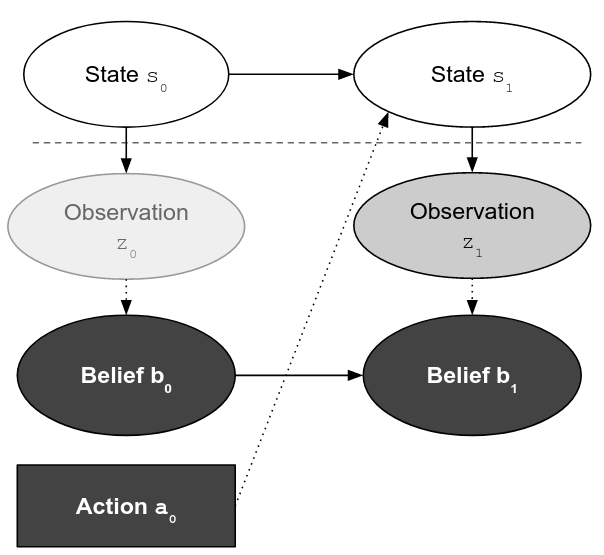
\includegraphics[width=0.5\linewidth]{figures/pomdp-state.png}
    \caption{A general process of a POMDP. True states are not available, instead, observations are received. These allow to update the agent's belief of the state that is used to choose an action to change the state towards a desired goal.}
    \label{fig:pomdp}
\end{figure}

A partially observable Markov decision process (POMDP) extends a Markov decision process (MDP) such that the agent does not directly observe the state of the environment and instead receives (partial) observations of the state.

Similar to an MDP, the state space $S$ describes the state of the environment, the action space $A$ is the set of possible actions the agent can take, the reward function $R(s, a)=r$ describes the outcome for the agent after taking an action $a \in A$ in state $s \in S$, and the transition model $T(s'|s,a)$ gives the conditional probability of the environment transitioning from state $s$ to state $s' \in S$ after the agent has taken action $a \in A$.
$\gamma \in [0,1]$ is a discount factor that describes how important future rewards are in comparison to immediate rewards when calculating total rewards.

In a POMDP, as the states are not directly available to the agent, the set of possible observations of the environment are denoted $z \in Z$ and the conditional observation model $O(z|s',a)$ assigns a probability of receiving the observation $z$ after taking action $a$ causing a transition to $s'$.
To track the state of the environment, the agent maintains a probability distribution over the state space $S$ called the belief $b$.
$b(s)$ is the probability the agent assigns to the state $s$ matching the environment's state.
Through a series of observations, the agent can update this belief to infer the state of the environment.
The goal of the agent is to find an action sequence that maximizes the expected discounted future rewards $E\left[\sum_{t=0}^\infty \gamma^t r_t \right]$ where $t$ denotes the time step of the interaction and $r_t$ is the reward at that step. 

Figure \ref{fig:pomdp} describes the interaction in a POMDP. 
Taking an action $a_0 \in A$ causes a transition of the environment's state from $s_0$ to $s_1$ with probability $T(s_1|s_0,a_0)$. 
Then, the agent receives the observation $z_1$ with probability $O(z_1|s_1,a_0)$ and a reward $r_1=R(s_1,a_0)$.
This enables the agent to update its belief from $b_0$ to $b_1$ as described in the next section.
%With a correct model of the environment and an intelligent agent, the probability of the correct state under the belief should increase $b_1(s_1) \geq b_0(s_0)$.

\subsubsection{Belief update}

We denote the operation of updating the belief from $b$ to $b'$ as $\tau(b,a,z)$.
%It depends only on the previous belief, the current action, and the current observation because the state is assumed to be Markovian.
A generic belief update can be described with Bayesian statistics.
For discrete states, the probability of a single state can then be updated using the formula:
\begin{equation}
    b'(s') = \eta \cdot O(z|s',a) \sum_{s \in S} T(s'|s,a) \cdot b(s)
    \label{eq:belief}
\end{equation}
where $\eta$ is the normalization term $1 / \sum_{s'} b'(s')$ to assert its sum is $1$.
%as the probability distribution must sum up to $1$. 
This formula must be applied to every state $s \in S$ to obtain the updated belief $b'$.
The complexity of a full belief update is then of order $O(|S|^2)$.

\subsubsection{Application to automated teaching}

This formulation can be applied to automated teaching as follows: the student represents the environment and the knowledge of the student is modeled as the state $s \in S$ that is hidden from the teaching program.
The automated teacher is the agent operating in this environment by choosing actions $a \in A$ to teach the topic.
The student responds to actions with answers $z \in Z$ that represent the observations for the automated teacher.
The automated teacher maintains a belief $b$ as a probability distribution of the knowledge of the student.
In general, its goal is to change the state of the student such that the student has mastered the topic %, although this depends on the task and context.
according to the reward function according to the pedagogical objective(s).
The original formulation by Rafferty \textit{et al.} simplifies the reward function to only depend on the action $R(a)$.

If the student's learning behavior is known, the teacher can plan and choose actions in such a way that the learning of the student is optimized. 
Such a model would thus define the transition and observation functions needed to apply the POMDP framework.


Rafferty \textit{et al.} consider that an action $a$ is the choice of a specific type of \textit{teaching activity} $t \in T$ (type) \textit{and} a specific \textit{teaching item} $i \in I$ that describes some content or example of the topic.
This decomposition allows simplifying the formulation when different teaching methods are available.
See section \ref{sec:concept-learning} for more details.


\subsubsection{Planning optimal actions}
\label{sec:planning}

Finding a policy that optimizes the pedagogical objective(s) is done via online planning, i.e., during execution. Offline planning, i.e., precomputing best actions for every possible belief state, might become computationally expensive and, thus, not tractable for longer trials or teaching tasks with a large state space. 
Hence, Rafferty \textit{et al.} employ a forward tree search algorithm with a finite horizon similar to Ross \textit{et al.}~\cite{rossPomdp2008}.

In a nutshell, the process is as follows:
The forward search starts from the current belief state $b$. 
A set of actions $\Tilde{A} \subset A$ is sampled to lower the computational cost.
Their values $q$ are calculated by simulating an interaction until horizon $d$ (depth) and the action $a^* \in A$ with the highest value is selected by the automated teacher.
%Note that we follow the convention from reinforcement learning literature to denote state values with $V$ and state-action values with $Q$.

Thus, we compute the best action $a^*_d(b)$ for a fixed horizon as follows:
\begin{equation}
    a^*_d(b) = \arg \max_{a \in \Tilde{A}} Q_d(b, a)
    \label{eq:best-action}
\end{equation}
with $b$ the current belief state, $d \in \mathbb{Z}$ the search depth, $\Tilde{A} \subset A$ the sampled actions, and $Q_d(b, a)$ the action-value function for action $a$ under the belief $b$ calculated until $d$. This follows the common notation in reinforcement learning where action-value functions are used to denote the expected reward when performing a particular action in a given state.


Since actions are composed of items $i \in I$ and teaching activity types $t \in T$, the action sampling is decomposed as follows:
$n$ teaching items $\Tilde{I} \subset I$ are sampled and the cartesian product with all teaching activity types $T$ is constructed to create $\Tilde{A} = \Tilde{I} \times T$.
The number of sampled actions is then equal to the product of sampled items and number of teaching types $|\Tilde{A}| = n \cdot |T|$.
This prevents ending up with actions of only a few types, which is very probable in the case of $|I| \gg |T|$.

A single action $a$ might cause different state changes according to $T(s'|s,a)$, and thus, different observations $z$.
For each action-observation pair, a new belief $b'=\tau(b,a,z)$ is computed.
With this new belief, the process starts anew: new actions are sampled and evaluated.
The forward search expands tree-like and grows exponentially in breadth.
To keep the computations tractable, the search is limited by a fixed depth and a reduced sample size.

% Lukas: In some way, it could be formulated to a more generic case where the empty response is part of the set of valid responses and in all cases the set is iterated but the probability of the responses result in the same result (as 0 prob for invalid responses).
If the set of possible observations following an action depends on the type of teaching activity associated with that action, we can simplify the calculation to only consider those observations that are possible for that teaching activity $Z_{i_a} \subset Z$.

To calculate the value of an action under the current belief, the future expected values of all possible observations for that action need to be considered and added to the value of the action itself. 
We compute $Q_d(b, a)$, the expected value for using the action $a \in A$ in the belief $b$ with search depth $d$ as:

\begin{equation}
    Q_d(b, a) = \begin{cases}
        R(a) + \sum_{z \in Z_{i_a}} Pr(z|b,a) \cdot \gamma \cdot V_{d-1}(b' = \tau(b, a, z)) & \, \text{if $d > 0$} \\
        \Hat{V}(b) & \, \text{if $d = 0$}
    \end{cases}
\end{equation}
with
$R(a)$ the reward for action $a$,
$Pr(z|b,a)$ the probability of receiving $z$ for action $a$ under the belief $b$,
$\gamma \in [0, 1]$ the discount factor, 
$V_d(b')$ the value function for the new belief,
and
$\Hat{V}(b)$ an estimation function of the value of the belief $b$ when the search depth is reached. 

The value of the belief $V_d(b)$ is defined as the maximum of the action-values $Q_d(b,a)$ for search depth $d$ over the sampled actions $\Tilde{A}$:
\begin{equation}
    V_d(b) = \max_{a \in \Tilde{A}} Q_d(b, a)
\end{equation}

Further, the probability of receiving an observation for an action under a belief $Pr(z|b,a)$ is simply the sum of the observation model $O(z|s,a)$ for every state, weighted by the belief probability of that state $b(s)$.
\begin{equation}
    Pr(z|b,a) = \sum_{s \in S} b(s) \cdot O(z|s,a)
\end{equation}


Finally, when the depth $d$ is reached, the value of the belief state at the leaf node is estimated by $\Hat{V}(b)$.
The specific estimation function thus needs to be defined by the task implementation of the method (see section \ref{sec:concept-learning}).
The estimated leaf value is propagated back up and discounted according to $\gamma$. 

The value of an action under a belief at a certain depth $Q_d(b,a)$ is thus the sum of the immediate reward of the action $R(a)$ and the sum over all valid observations for that action $Z_{i_a}$ of the discounted back-propagated belief state values $\gamma \cdot V_{d-1}(b')$, weighted by the observation probability $Pr(z|b,a)$.
According to the values of a set of actions, the best action $a^*_d(b)$ can be chosen according to \autoref{eq:best-action}.

%%% Lukas: Is the algorithm understandable?
\begin{algorithm}[ht]
\SetAlgoLined
\DontPrintSemicolon
\SetKwData{Input}{Data}
\KwIn{\\
\begin{tabularx}{\textwidth}{p{0.45cm}l}
    $b$      & current belief\\
    $n$      & no. of samples per level\\
    $d$      & horizon
\end{tabularx}
}
\KwOut{\\
\begin{tabularx}{\textwidth}{p{0.45cm}l}
    $v^*$     & best value of next action \\
    $a^*$     & best action
\end{tabularx}
}
\SetKwFunction{forwardsearch}{ForwardSearch}
\SetKwProg{Fn}{Function}{:}{}
\Fn{\forwardsearch{$b, n, d$}}{

$\Tilde{I} \leftarrow$ sample $n$ items uniformly from $I$\;
$\Tilde{A} \leftarrow$ $\Tilde{I} \times T$\;

$v^* \leftarrow \infty$\;

\For{$a \in \Tilde{A}$}{
    $q \leftarrow R(a)$\;
    
    \For{$z \in Z_{i_a}$}{
        $b' \leftarrow \tau(b, a, z)$\;
        
        % Lukas: It makes it easier to write the condition at this point
        % instead of in the beginning with d = 0. But this now differs from the equation formulation. Is that still okay?
        \eIf{$d = 1$}{
            $v \leftarrow \Hat{V}(b')$\;
        }{
            %%% Lukas: not sure how to represent that we only take the value
            $v \leftarrow v^*$ of \forwardsearch{$b', n, d-1$}\;
        }
        
        
        $q \leftarrow q + Pr(z|b, a) \cdot \gamma \cdot v$\;
    }
    
    \If{$q > v^*$}{
      $v^* \leftarrow q$\;
      
      $a^* \leftarrow a$\;
    }
}

\KwRet{$v^*$, $a^*$}
}
 
 \caption{Recursive forward search planning algorithm}
 \label{plan-algo}
\end{algorithm}



This algorithm is described in \autoref{plan-algo}.
It is implemented as a recursive algorithm that returns the maximum expected reward of the next action and the best action according to this reward.
In intermediate calls, the best value is used to calculate the value of the immediate action while at the top level the best action is used to define the next action to take.
For simplicity, we describe it with a single best action although in practice it is useful to maintain a list of actions with the highest known reward and choose the next action from that list. This is to prevent biasing the method toward some internal structure of the actions.

\subsection{Application as ``faster teaching'' to concept learning}
\label{sec:concept-learning}

The authors apply this general formulation to concept learning tasks.
Category or concept learning is the process of learning categories from examples~\cite{feldman2003simplicity}.

In such tasks, we denote the set of concepts as hypotheses $H$.% to better distinguish them from costs. 
The task description has to be complemented with (i) a prior distribution $p_0$ over these concepts, (ii) the items that can be used to teach the task $i \in I$, (iii) the teaching activities $t \in T$, and (iv) the possible responses $Z$.

The reward function is defined such that the teacher focuses on reducing the time needed for learning the task, hence the name ``faster teaching''. 
Each teaching action is associated with a cost (negative reward) that is modeled after the time it takes the student to complete the action. 
Thus, minimizing the costs results in the quickest learning. 
We use the cost of an action $C(a)$ and a minimization objective instead of maximizing rewards (if $R(a) = -C(a)$, then $\arg \max_a R(a) = \arg \min_a -R(a)$).

Teaching is terminated once the student has learned the concept. This is assumed if in an assessment phase the learner answers all questions correctly.
Such an assessment is performed at regular intervals to check for termination, but not used for updating the beliefs of the teacher.

\subsubsection{Teaching activity types}

In the context of concept learning, Rafferty \textit{et al.} define three possible types of teaching activity $T$: (1) showing an \textit{example}, (2) asking a \textit{quiz}, and (3) asking a question and subsequently giving \textit{feedback} about the student's response. 

\paragraph{(1) Example} In an example, the teacher presents an item with the correct result or concept. No response by the student is expected. Thus, $Z_{\text{example}} = \{\emptyset\}$. The observation model is trivial: $O(z|s,a)=1$ if $z=\emptyset$ and $0$ otherwise. However, as the example can provide new insight for the learner, the transition model assumes a state change for such cases. This change depends on the learner model and is described in the next section.

\paragraph{(2) Quiz} In a quiz, the teacher presents an item and the student has to respond with an answer.
%(in the arithmetic letter task with the correct result, and in the game number with the correct concept)
This allows the teacher to refine their belief about the student's true state, but it does not give new information to the student. 

The set of observations for this activity type contains the full set of observations valid for the concept task, $Z_{\text{quiz}} = Z$.
The definition of the observation model $O(z|s,a)$ depends on the learner model and is described in the next section. 
The transition model $T(s'|s,a)$ is trivial: as no new information is presented, the student is not expected to change their state. The transition probability is set to $1$ if both states are the same, $0$ otherwise.

\begin{equation}
    T(s'|s,a) = \begin{cases}
        1 & \, s  = s' \\
        0 & \, s \neq s'
    \end{cases}
\end{equation}

As a result, $\sum_s{T(s'|s,a) b(s)}$ of the belief update in \autoref{eq:belief} collapses to just $b(s')$.

\paragraph{(3) Feedback} In a question with feedback type of teaching activity, the previous types are combined. First, the learner is asked a question to which they respond according to their knowledge. Then, the teacher reveals whether the response was correct, and gives the correct answer in case of an incorrect answer. 
Here, both the observation model and the transition model are used in a non-trivial way. 
As in the \textit{quiz}, the set of observations for this teaching activity contains the full set of observations valid for the concept task, $Z_{\text{feedback}} = Z$, and the observation model $O(z|s,a)$ depends on the learner model. 
And as in the \textit{example}, the transition model depends on the learner model, as the feedback can provide new information to the learner.

Note that when modeling the update as in the Bayesian belief formula (\ref{eq:belief}), the update has to be split into two separate steps: the response of the learner is always related to the state before taking the action, while the feedback might trigger a state change without an additional observation. So first, the belief update according to the response $z$ has to be calculated in the same way as in the \textit{quiz} activity. Second, if the response was incorrect, a state change is expected based on the true answer, as in the \textit{example} activity type.

\vspace{3mm}
To reflect these similarities between the feedback type and the other activity types, we will use \textit{refinement activities} to refer to the quiz activity and the question part of the feedback activity (as they both allow the teacher to refine the belief), and \textit{evidence activities} to refer to the example activity and the feedback part of the feedback activity (as they both allow the learner to improve its knowledge). 

We define the generic belief update formulas for \textit{refinement} and \textit{evidence activities} as:

\begin{equation}
    b'(s') = \begin{cases}
        \eta \cdot O(z|s',a) \cdot b(s')    & \, \text{for refinement activities} \\
        \eta \cdot \sum_{s \in S} T(s'|s, a) \cdot b(s)    & \, \text{for evidence activities}
    \end{cases}
    \label{eq:belief-update-types}
\end{equation}

$\eta$ refers to the normalization term and depends on the belief formula.

Finally, we denote by $H_a$ the set of concepts (hypotheses) that are consistent with action $a$, and $H_{z \mid a}$ the set of concepts which imply that $z$ is a correct answer to action $a$. 

\subsection{Learner models}

The learner model defines the details of the transition and observation functions.
Rafferty \textit{et al.} postulate three learner models: (1) a discrete memoryless model, (2) a discrete model with memory, and (3) a continuous model with a dynamic probability distribution over the concept space. All models are extended to include noise to accommodate human error during the learning.


\paragraph{Noise} Two types of noises are added to all models: a production noise $\epsilon_p$ for cases where the student responds inconsistently to their knowledge, and a transition noise $\epsilon_t$ for cases where the student ignores new evidence and does not transition to a new consistent state.
For the production noise, it is assumed that the student responds with a random answer drawn uniformly from all possible answers. 
The transition noise affects the state transitions, and the models need to incorporate this behavior in their updating rules to prevent diverging beliefs and states.

\paragraph{(1) Memoryless model}
This model is close to the learning model of Restle \textit{et al.} \cite{restle1962selection} and assumes that no explicit memory of previous actions is kept while storing a specific concept hypothesis that is currently believed to be true by the learner (as opposed to considering multiple possible plausible concepts).
Thus, the learner state only depends on the current knowledge and the immediate teaching activity.
The state space $S$ is isomorphic to the space of possible concepts $H$, such that any $s\in S$ corresponds to one specific concept hypothesis denoted $h_s$.

For refinement activities, the observation model needs to be defined.
As the learner holds a single true concept, the response corresponds to the result under this single concept.
Taking noise into account, the observation model is defined as follows:
\begin{equation}
    O(z|s,a) = \begin{cases}
        (1-\epsilon_p)+\frac{\epsilon_p}{|Z_{i_a}|}    & \, \text{if $z$ is consistent for $a$ under $s$} \\
        \frac{\epsilon_p}{|Z_{i_a}|}                   & \, \text{otherwise}
    \end{cases}
\end{equation}
with $\frac{\epsilon_p}{|Z_{i_a}|}$ the probability of choosing a random response in case of a production error.


For evidence activities, the learner is assumed to transition to a concept consistent with the new evidence if not already in a consistent state. The probability of each consistent concept is proportional its prior probability. 
% Lukas: removed as not necessary really, right? We can go directly to the noisy definition
% \begin{equation}
%     T(s'|s,a) \propto
%     \begin{cases}
%         p_0(h_{s'}) & \, \text{if $h_{s'} \in H_{a}$} \\
%         0       & \, \text{otherwise}
%     \end{cases}
% \end{equation}
% with $p_0$ the prior probability over the possible concepts.
With noise, the transition model is defined as follows:
\begin{equation}
    T(s'|s, a) = \begin{cases}
        1       & \, \text{if } h_{s'} \in H_a \text{ and } s' = s, \\ %s'=s consistent, already in the same consistent state
        (1 - \epsilon_t) \cdot \dfrac{p_0(h_{s'})}{\sum_{s'' \mid h_{s''} \in H_a} p_0(h_{s''})} & \, \text{if } h_{s'} \in H_a \text{ and } s' \neq s, \\ %s' consistent, s inconsistent
        \epsilon_t & \, \text{if }  h_{s'} \notin H_a \text{ and } s' = s, \\ %s'=s inconsistent
        0 & \, \text{otherwise}
    \end{cases}
    \label{eq:trans-model}
\end{equation}
with $p_0$ the prior probability over the possible concepts,
and $\frac{p_0(h_{s'})}{\sum_{s'' \mid h_{s''} \in H_a} p_0(h_{s''})}$ the probability of going from an inconsistent state to a particular consistent state based on the relative prior among the consistent states.

%This implies that the learner stays with probability $\epsilon_t$ in states inconsistent with the new evidence provided by the action.

The sum over states in \autoref{eq:belief-update-types} for evidence actions can be decomposed to accommodate this structure.
For states consistent with the information provided by the action, it is composed of two parts: the likelihood of transitioning from an inconsistent state to this consistent state, and the likelihood of already being in this state and, thus, not transitioning.
The belief update is consequently:
\begin{equation}
    b(s')= \begin{cases}
        \eta \cdot \left[(1 - \epsilon_t) \cdot \frac{p_0(h_{s'})}{\sum_{s \mid h_s \in H_a}{p_0(h_s)}} \cdot \sum_{s \mid h_s \notin H_a}{b(s)}\right] + b(s') & \text{if } h_{s'} \in H_a \\
        \eta \cdot \epsilon_t \cdot b(s') & \text{ otherwise }
    \end{cases}
\end{equation}

Note, that in case of feedback activities, the evidence update only has to be performed for incorrect answers, as the learner is assumed to not transition for correct responses.


\paragraph{(2) Discrete model with memory}
%%% Lukas: Actually, there is no reference for this model cited in the original paper
This model extends the memoryless model so that a history of the past $m$ actions is kept.
Transitions then have to be consistent with the current action plus the memory actions, denoted $A_M$.
The memory only needs to store actions that contain information, i.e., quiz activities are ignored.
As for the memoryless model, it is assumed that the student only holds a single concept as true and responds accordingly to it.


If the memory would not be perfect, it must be considered part of the student's state.
In this case, the number of possible memory states $S_M$ is calculated based on the set of teaching items $I$ and the set of valid memory teaching activities $T_{mem}$ as $|S_M| = \sum_{k=0}^m |I \times T_{mem}|^k$.
%While $|I \times T_{mem}|^m$ represents the memory states where all slots are filled, the lower powers represent those states where some slots are not filled which can only occur on one side.
Taken together, the total state space would increase by the memory states and become $|S|=|H| \cdot |S_M|$ resulting in a possibly huge state space.
For example, in the letter arithmetic task with 6 letter-number pairs, 15 teaching items, 2 valid memory teaching activities, and a memory size of $2$, the total number of memory states would grow from $|H|=720$ to $|H|\cdot (1 + 30 + 30^2) =670.302$.


However, the model assumes a `flawless' memory, i.e., even if an action is ignored for updating the state due to the transition noise, it is kept in memory. As a consequence, at every time step, only the single memory state based on the action history is possible and needs to be considered, reducing the state space to $|H|$ as before.

The transition and observation models are formulated analogously to the memoryless case. 
The only difference is that the set of consistent concepts with the current action $H_a$ has to be consistent also with the actions in memory $A_M$.

\paragraph{(3) Continuous model}
This model assumes that the student maintains a probability distribution over all possible solutions as formulated in \cite{tenenbaum2000rules}. 
No explicit history of previous actions is stored but the state contains implicit information about the history.
In this case, every state is a probability distribution over all elements of $H$, making the state space infinitely large. Thus, approximations are needed to make this model feasible.

In this model, a state consistent with an action-observation pair is one in which the probabilities of all inconsistent concepts with the action is zero $p_s(h \notin H_a) = 0$.

Responses to teaching actions are probabilistic and correspond to the combined probability the student places on the concepts with $z$ as a correct answer.

\begin{equation}
    O(z|s,a) = \sum_{h \in H_{z \mid a}} p_s(h)
\end{equation}

where $p_s(h)$ is the probability of the hypothesis $h$ in the state $s$.

The transition model is defined such that for new evidence, the learner transitions deterministically to the closest consistent derivation of the current state $s$.
This derived state $s_a^*$ for the current action $a$ is a copy of the current state in which the probabilities of all inconsistent hypotheses are set to $0$ while the other probabilities are retained and normalized.

\begin{equation}
    T(s'|s,a) = \begin{cases}
        1     & \, \text{if $s$ is consistent with $a$ and $s' = s$} \\
        1     & \, \text{if $s$ is inconsistent with $a$ and $s' = s_a^*$} \\
        0     & \, \mathrm{otherwise}
    \end{cases}
    \label{eq:cont-ps}
\end{equation}

With diverse evidence, the probability distribution converges to the true concept.

From the perspective of the teacher, it is intractable to hold a belief over the infinite set of states. Below, we review the particle filter implementation that is employed instead.

\paragraph{\textit{Particle filter}}
A particle filter is used to approximate the infinite set of possible states via a limited number of weighted particles \cite{DoucetSeqMCM2001}.
In this particle filter, each particle $p \in P$ represents one possible state $s_p$ (i.e., a probability distribution over concepts), and the weight $w_p$ indicates the probability the teacher assigns to this particle.
The sum of the weights must always be $1$ as in a probability distribution.
The particles $P$ can be thought of as corresponding to $b$ and the weights to $b(s)$ in the discrete case.
As the belief state is approximated, the belief update $\tau(b,a,z)$ is now a function of the existing particles as described below.

In the beginning, the particles are initialized with two particles sharing equal weight: one particle corresponding to the prior distribution $p_0$, and one particle with a uniform distribution over the concepts. 
If the prior distribution is uniform, only one particle is created.

After each action, the particles are updated, and new particles are created based on the observation and transition models, and their weights are recalculated.
This corresponds to the belief updates in the discrete models.

For \textit{refinement activities}, the weights of the particles are updated based on the observation model as follows:

\begin{equation}
    w_p' = \eta \cdot w_p \cdot O(z|s,a)
\end{equation}

\begin{equation}
    O(z|s,a) = (1 - \epsilon_p) \cdot \sum_{h \in H_{z\mid a}}{p_{s_p}(h)} + \frac{\epsilon_p}{|Z_{i_a}|}
\end{equation}
with $\frac{\epsilon_p}{|Z_{i_a}|}$ being the probability of observing the response $z$ due to a production error.
$\eta$ now refers to the renormalization factor after processing all particles, $1 / \sum_{p \in P}{w_p}$.
This corresponds to the regular belief update \autoref{eq:belief-update-types}.

For actions using an \textit{evidence activity}, every particle is replaced by two new particles, one assuming the learner did not transition, and one assuming the learner transitioned.
The non-transitioned particle is simply a copy of the previous particle, with the weight adjusted by $\epsilon_t$.
The transitioned particle is based on the old particle and updated to reflect the new evidence. For this, the probability for all inconsistent states is set to zero $p_{s_p}(h \notin H_a) \leftarrow 0$.
The weight of both particles is thus updated according to:

\begin{equation}
    w_p' = \begin{cases} 
        \eta \cdot (1 - \epsilon_t) \cdot w_p & \, \text{for transitioned particles} \\
        \eta \cdot \epsilon_t \cdot w_p & \, \text{for non-transitioned particles}
    \end{cases}
\end{equation}

Since this update doubles the number of particles, there is a limit imposed to prevent uncontrolled growth on the number of particles.
If the total number of particles exceeds some predefined maximum, the particles with the smallest weight are removed so that the limit is satisfied, and the weights are normalized again.


The weight updates and renormalizations are performed after both \textit{refinement} and \textit{evidence} activities separately (relevant in the case of \textit{feedback} activities).
Further, in both cases, there is a check for \textit{particle depletion} (i.e., no particle is probable).
This happens if the sum\footnote{Note that it is always the \textit{sum} and not the maximum of the weights as wrongly stated in one passage in the original supplementary material (as confirmed from the original implementation).} of all particle weights is below some threshold.
In this case, all particles are eliminated, and two new particles are initialized with equal weight.
One particle is created according to the prior distribution and the other particle according to the state a learner without noise would have ended up in following the history of previously seen actions. 

In this model, the update based on new evidence has to be done also for correct responses to feedback activities, as the response is sampled from the state of the learner and does not represent a certain answer.

\subsubsection{Planning}

For every learner model, a corresponding policy is constructed that follows the forward tree search planning algorithm described in section \ref{sec:planning}.
To estimate the cost of the leaf nodes in such concept learning tasks, 
the authors take the probability of failing the assessment phase (given by the belief) and multiply it by a scaling of the minimum future costs:

\begin{equation}
    \Hat{V}(b) = (1 - p_b(h_{true})) \cdot \alpha \cdot \min_a{C(a)}
    \label{eq:leaf-calc}
\end{equation}
with $p_b(h_{true})$, the probability assigned to the true concept in the current belief, and $\alpha$ a scale parameter. 

For the memoryless and the model with memory, $p_b(h_{true})$ is simply the belief probability of the true concept. 
For the continuous model, it is the combined probability of the true concept of all particles, weighted by the corresponding particle weight.

\begin{equation}
    p_b(h_{true} \mid b) = \begin{cases}
        b(s = h_{true}) & \, \text{for the discrete models} \\
        \sum_{s_p \mid p \in P}{w_{s_p} \cdot p_{s_p}(h_{true})} & \, \text{for the continuous model}
    \end{cases}
\end{equation}

\subsection{Comparison with original paper}

We tried to honor the original method description as much as we could.
While certain elements were not clear to us, we discussed open questions with the first author of the original paper, and verified certain assumptions with their implementation.
Specifically, we verified that one should compute the belief update without the explicit Bayesian equation (\ref{eq:belief}), and treat the belief update as a two-step process for the refinement and evidence parts of the actions, which is especially relevant for the \textit{feedback} activity.
% This led us to handle it as a combination of the other two activities.
We deduced the planning algorithm \ref{plan-algo} from the referenced papers and validated it with the original implementation, and verified that the memory is not part of the state in the discrete model with memory, and that the memory ignores quizzes.
% Finally, as well as the handling of noises in the learner models, and how they are treated in the respective equations.
As such, we did not have to take design decisions as clarifications were provided by the original authors.
Still, there might be differences in implementation details as we focused our validation on the conceptual algorithms and model equations.


\section{Experiments}
We applied our implementation to both concept learning task from the original paper: the \textit{Letter Arithmetic} task and the \textit{Number Game}. 
As we were interested in the method and its possible applications, we performed simulations only and no experiments with humans.
%What follows is a brief description of the tasks, our simulation approach and an explanation of our results.

\subsection{Baselines}

We compare the results to the baselines introduced in the original paper: a \textit{random} policy, a random policy with only quiz and example actions (\textit{quiz-example only/QE only}) and policy with planning according to \textit{maximum information gain (MIG)}.

% TODO check, filtering
The \textit{random} policy selects any of the $a \in A$ actions randomly, however, making sure that no item $i \in I$ is sampled twice in the same teaching phase.
%In the \textit{number game}, there are some further constraints that are applied to the randomness.


The \textit{quiz-example only} policy ignores the feedback activity.
It was introduced since in the first original experiment with the letter arithmetic task, the planning algorithms did not use any feedback actions, resulting in a much higher average cost for the random policy compared to the POMDP planners.

The \textit{maximum information gain} policy performs a single planning step with the continuous learner model. For every possible action, it simulates the belief change according to the continuous model and compares the Shannon entropy of the current and the new belief state.

\begin{equation}
    entropy(b)=\sum_{s_p \mid p \in P}{w_{s_p}} \cdot \left( -\sum_{h \in H}{p_{s_p}(h) \cdot \ln\left( p_{s_p}(h) \right)} \right)
\end{equation}

The planner selects the action which produces the highest information gain for the learner, i.e., the one that reduces the entropy the most.
As with the continuous policy, the particle filter approximation is employed, and thus, the entropy of the belief state is calculated as the weighted sum over the entropy of the particles.
This policy provides only example activities to teach a concept as refinement activities do not provide new information to reduce the entropy.
As such, it cannot understand errors during learning and revise its belief.


\subsection{Task 1: Letter Arithmetic}

The \textit{letter arithmetic} task is composed of addition equations with two letters, such as $A+B=3$. In the original experiments, the mapping length is set to 6, which corresponds to the letters A-F being mapped to the numbers 0-5 (we confirmed that there was a typo in one passage noting a larger range of numbers 0-6).

Some sample actions are thus: $B+F=5$ (example), $A+C=?$ (quiz) and followed by $correct$ or $answer=2$ for feedback actions. 
The number of possible teaching items $I$ can be reduced by only considering the possible combinations of the letters, i.e., ignoring order. For the case with 6 letters, this gives $|I|=15$ and a maximum $|I \times T|=45$ actions to evaluate.

The set of valid responses $Z$ are the numbers $1-9$.
During the assessment phase, the learner is queried to provide the correct mapping for each letter.
The estimation of the belief value of the leaf nodes $\Hat{V}(b)$ follows \autoref{eq:leaf-calc} with $\alpha=10$.
We use the original values for the cost function $C(a)$ and noise parameters, as shown in tables \ref{tab:action-cost-t1} and \ref{tab:noise-t1}, that were fitted from control experiments with users in the original study.

\begin{table}
\small
\parbox[t]{.49\linewidth}{
    \centering
    \begin{tabular}[t]{l|r}
        \hline
        \textbf{Teaching type} & \textbf{Cost} in seconds \\
        \hline
        Example & 7.0 \\
        Quiz    & 6.6 \\
        Feedback & 12.0 \\
        \hline
    \end{tabular}
    \caption{\textit{Letter arithmetic}: Teaching activity costs}
    \label{tab:action-cost-t1}
}
\hfill
\parbox[t]{.49\linewidth}{
    \centering
    \begin{tabular}[t]{l|rr}
        \hline
        \textbf{Learner model} & $\epsilon_t$ & $\epsilon_p$ \\
        \hline
        Memoryless  & 0.15 & 0.019 \\
        Discrete    & 0.34 & 0.046 \\
        Continuous  & 0.14 & 0.12 \\
        \hline
    \end{tabular}
    \caption{\textit{Letter arithmetic}: Noise parameters}
    \label{tab:noise-t1}
}
\end{table}


The concept space $H$ is composed of all permutations of the 6 letters mapped to 0-5, so $|H|= 720$. 
This is also the state space for the memoryless and discrete policy, as well as the particle size in the continuous policy.
All concepts are assumed to be equally likely, so a uniform prior $p_0$ over the concepts is used.


\subsection{Task 2: Number Game}

The second task is called \textit{Number Game} \cite{tenenbaum2000rules}. 
The goal in this task is to infer a specific number concept for the number range $1-100$. Such a concept can be either mathematical $H_{math}$, like odd, even, multiples of 5, etc., or a range based concept $H_{range}$, like 10-20 or 64-83.
The student is presented a number and is either told if the number belongs to the target concept (example and feedback activities) or is asked to provide this categorization (quiz and question activities).

The set of teaching items $I$ is the range of numbers $1-100$, resulting in $|I \times T|=300$ possible actions.
The set of possible responses $Z$ only contains two values: `inside' and `outside' the concept.
During the assessment phase, the learner is presented with 10 items and has to give 10 correct answers to display mastery of the concept and terminate the teaching.
Of these items, 5 are sampled from within the concept and 5 from outside the concept.

For $\Hat{V}(b)$ to estimate the belief value of leaf nodes, \autoref{eq:leaf-calc} with $\alpha = 10$ is used as before.
Again, we use the original values for the cost function $C(a)$ and noise parameters, as shown in tables \ref{tab:action-cost-t2} and \ref{tab:noise-t2}, that were fitted from control experiments with users in the original paper.


\begin{table}
\small
\parbox[t]{.49\linewidth}{
    \centering
    \begin{tabular}{l|r}
        \hline
        \textbf{Teaching type} & \textbf{Cost} in seconds \\
        \hline
        Example & 2.4 \\
        Quiz    & 2.8 \\
        Feedback & 4.8 \\
        \hline
    \end{tabular}
    \caption{\textit{Number game}: Teaching activity costs}
    \label{tab:action-cost-t2}
}
\hfill
\parbox[t]{.49\linewidth}{
    \centering
    \begin{tabular}{l|rr}
        \hline
        \textbf{Learner model} & $\epsilon_t$ & $\epsilon_p$ \\
        \hline
        Memoryless  & 0.25 & 0.14 \\
        Discrete    & 0.18 & 0.10 \\
        Continuous  & 0.21 & 0.15 \\
        \hline
    \end{tabular}
    \caption{\textit{Number game}: Noise parameters}
    \label{tab:noise-t2}
}
\end{table}

The exact concept space is more difficult to recover. Tenenbaum \textit{et al.} \cite{tenenbaum2000rules} originally described 5,083 possible concepts. Rafferty \textit{et al.} reported to use 6,412 concepts, but the exact definition is not given. 
We received the original unlabelled concept values from the original author, from which we reverse engineered 6,354 of the 6,412 concepts (the remaining 58 concepts were the same as other concepts, and as there were no labels, we considered them duplicates).
In addition to the original 5,083 concepts, the set of \textit{less probable mathematical concepts} $H_{math+}$ is added, e.g., ``multiples of 4 minus 1'' or larger multiples such as ``multiples of 25''.
Details of the concept space can be found in \autoref{tab:ng-concepts}.

The definition of the prior $p_0$ is following a hierarchical model as described in \cite{tenenbaum2000rules}. 
The mathematical concepts $H_{math}$ and $H_{math+}$ are assigned $\lambda$ of the probability and each class in turn is assigned half of this prior.
As both classes are a lot smaller than the range concepts, they are assigned the majority of the prior if $\lambda$ is not small.
Inside each class, the prior is shared uniformly: $p_0(h \in H_{math}) = 0.5 \cdot \lambda / |H_{math}|= \lambda / 168$ and $p_0(h \in H_{math+}) = 0.5 \cdot \lambda / |H_{math+}|= \lambda / 5048$. 

The remainder $(1 - \lambda)$ is shared among the number range concepts $H_{range}$ proportional to an Erlang distribution according to their interval size: $p_0(h \in H_{range}) \propto (|h|/\sigma^2) \cdot e^{-|h|/\sigma}$. This should capture the intuition that medium sized ranges are more likely than very big or very small ranges.

For the free parameters $\lambda, \sigma$, we use the same values as originally described in \cite{tenenbaum2000rules}: $\lambda = 1/2, \sigma = 10$. 
That means, all mathematical concepts are assigned a prior probability of $1/168 \approx 5.95 \cdot 10^{-3}$, the less probable mathematical concepts a prior of $1/5048 \approx 1.98 \cdot 10^{-4}$, and e.g. the range 1-100 is assigned the prior $\approx 3 \cdot 10^{-7}$ while the range 64-83 a prior of $\approx 1.67 \cdot 10^{-4}$. 

As the less probable mathematical concepts $H_{math+}$ were reverse engineered, the corresponding prior was similarly deduced to best match the associated prior given by the original authors.
Still, these priors slightly differ 5-10\% from our reported values. On the one hand, this is because our space is smaller by 58 items but also because they might have used a slightly different $\lambda$ (for instance, a value around $0.55519$ instead of $1/2$ could explain this difference but it does not change the results significantly).

\begin{table}
\centering
\small
\begin{tabular}{l|r|r}
    \hline
    \textbf{Concept class}  & \textbf{Number of concepts} & \textbf{Prior} \\
    \hline
    \textit{Mathematical concepts (below)} & \textit{42} & $\sum = 1/4$ \\
    \hline
    Odd, even               & 2     & $1/168 \approx 0.0059524$ \\
    Square, cube            & 2     & $1/168$ \\
    Primes                  & 1     & $1/168$ \\
    Multiples of 3-12       & 10    & $1/168$ \\
    Powers of 2-10 (incl. 1)& 9     & $1/168$ \\
    Powers of 2-10 (excl. 1)& 9     & $1/168$ \\
    Numbers ending in 1-9   & 9     & $1/168$ \\
    \hline\hline
    \textit{Less probable mathematical concepts (below)} & \textit{1262} & $\sum = 1/4$ \\
    \hline
    Multiples of 13-50        & 38 & $1/5048 \approx 0.0001981$ \\
    Multiples of 3-50 minus $1...n-1$ & 1224 & $1/5048$ \\
    \hline\hline
    \textit{Ranges n-m}, $1 \leq n \leq 100, n \leq m \leq 100$ & \textit{5,050} & $\sum = 1/2$ \\
    \hline
    E.g. Range 10-20        & 1 & $\approx0.0002262$ \\
    E.g. Range 64-83        & 1 & $\approx0.0001672$ \\
    E.g. Range 1-100        & 1 & $\approx0.0000003$ \\
    ... & &                     \\
    \hline\hline
    \textbf{Total concepts} & \textbf{6,354} & $\sum = 1$ \\
    \hline
\end{tabular}
\caption{Set of concepts for the number game and their corresponding priors.}
\label{tab:ng-concepts}
\end{table}

Finally, the two random policies' sampling strategy is modified such that with 50\% probability an item inside the concept, and otherwise outside the concept is sampled.
This was introduced after the original authors noticed that a completely random policy was too frustrating for the human learners.

\subsection{Simulation}

We validated our implementation by running the same simulations as in the original paper. 
Every planning policy was tested with every learner model simulation. 
Hence, for every simulated learning model, the three baselines and the three planning policies with the learning models were tested, leading to a total of 18 pairings.
Those pairs were run 50 times each with a different but controlled seed set for the random number generators. In all trials of the same pair, the task instance was the same. 
The horizon depth and samples per level were the same as in the original paper.

In the \textit{letter arithmetic} task, all models used a horizon of $d=2$. 
The memoryless model sampled 7 items in the first level and 6 in the second level. The discrete model with memory sampled 8 items in both levels, and the continuous model sampled respectively 4 and 3 items.
Teaching phases consist of three actions followed by an assessment phase. After a maximum of 40 teaching phases (i.e., 120 total actions) and a failed assessment phase, the learning was terminated without success.

In the \textit{number game}, the memoryless model and the discrete model used a horizon of $d=2$, with 6 and 8 items sampled, and 6 items sampled in both levels respectively. The continuous model had a horizon of $d=3$, with 6, 6 and 8 items sampled. 
Teaching phases lasted 5 actions. The maximum number of teaching phases was again 40 (i.e., 200 total actions).

In both tasks, the memory model was using a memory size of 2, and the continuous model's maximum particle size was set to 16 with the particle depletion threshold of 0.005, as in the original experiments.
% try in a big table everything

\subsubsection{Precomputing actions}
The authors note that for computational reasons, they precomputed the first actions and cached them to be used in all trials. During this precomputation, 10 items were sampled per level.
The original paper reports only this number for the first task, but we used the same number for the second task. In the \textit{letter arithmetic} task, 9 actions were precomputed, while in the \textit{number game}, 20 actions were precomputed.
Also, the same horizon as the target policy is used in every step.

Through precomputing actions, possibly better starting points would be found. Naturally, during precomputation, the true responses of the learners are not known.
If an action with a non-empty response set is returned as the best action, a separate branch for every possible response has to be followed.
This ensures that during teaching, the corresponding path according to the learner's response is available.
This leads to a possibly very large number of branches.

\subsubsection{Evaluation metric}

To compare our replication, we use the same metric as in the original study to evaluate the planning policies for each simulated learner, the \textit{median time to mastery}.
This refers to the hypothetical time the simulated learner spends with the automated teacher based on the time cost of each action type.

For example, in the letter arithmetic task, if a learner is shown three examples and one quiz, the expected time to mastery is $27.6$. 
Note that assessment phases are not taken into consideration in the time calculation.
If mastery is not achieved, the total time spent until this point is used. 
As each teaching phase consists of 3 actions and the least costly activity is the quiz, the theoretical minimum time is $19.8$ (although it is impossible to learn only via quizzes), and the maximum time would be $1440$. 
In a setting using only examples, the minimum time would be $21.0$, while for maximum runs, averaging over the action costs, the time until termination is expected to be $1024$.


For the number game, the action costs are much smaller, while the teaching phases are longer.
The theoretical minimum time is $12.0$ using example activities.
The averaged maximum in this task is then $\approx 666.67$.

These numbers allow us to get an intuition of how well a learner is doing in respect to the bounds of the problem.

\subsection{Results}

\subsubsection{Letter Arithmetic}

% \begin{figure}
%     \centering
%     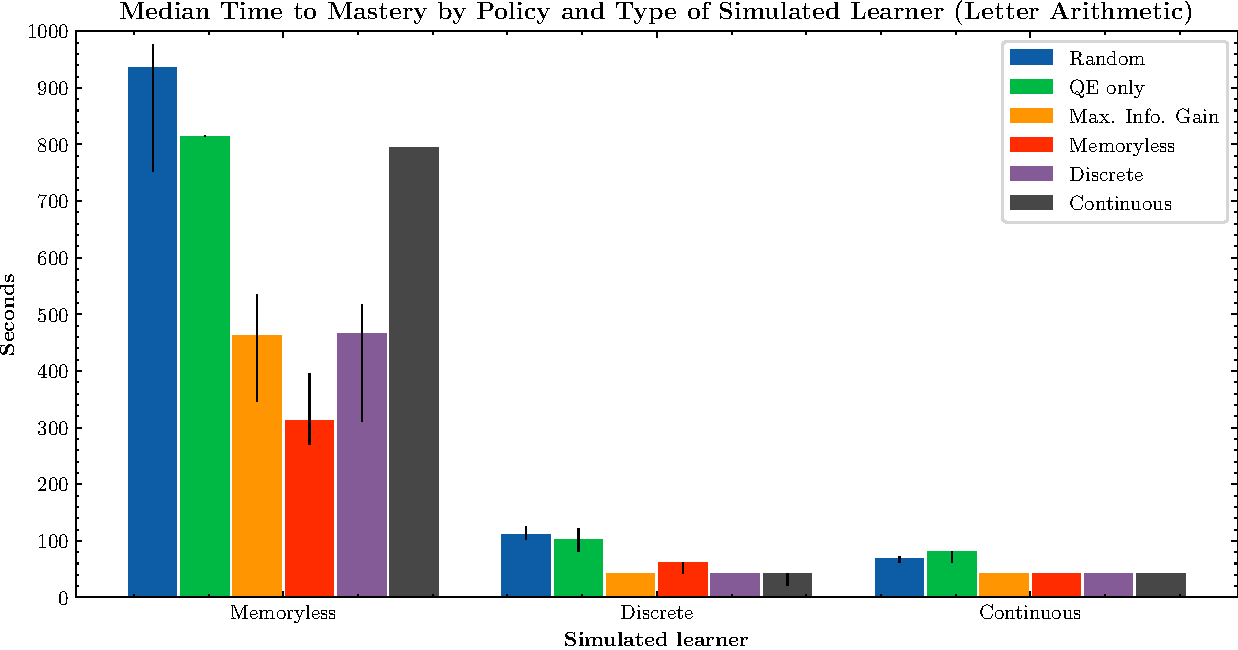
\includegraphics[width=\linewidth]{median-time-letter.pdf}
%     \caption{Median time to mastery for the letter arithmetic task. The results are grouped for each simulated learner (x axis) showing the performance of the different policies. The error bars represent the bootstrapped 68\% confidence interval. Replication of figure 4 from the original paper.
%     %The results are similar as well. Our results differ for the simulated memoryless learner which achieves a significantly better score for the memoryless planning model, and a worse score for the discrete memory planning model. Both the simulated learners with discrete memory and the continuous model achieve the same near minimum results with 42.0s, corresponding to two teaching phases with examples.
%     }
%     \label{fig:median-time}
% \end{figure}


% \begin{figure}
%     \centering
%     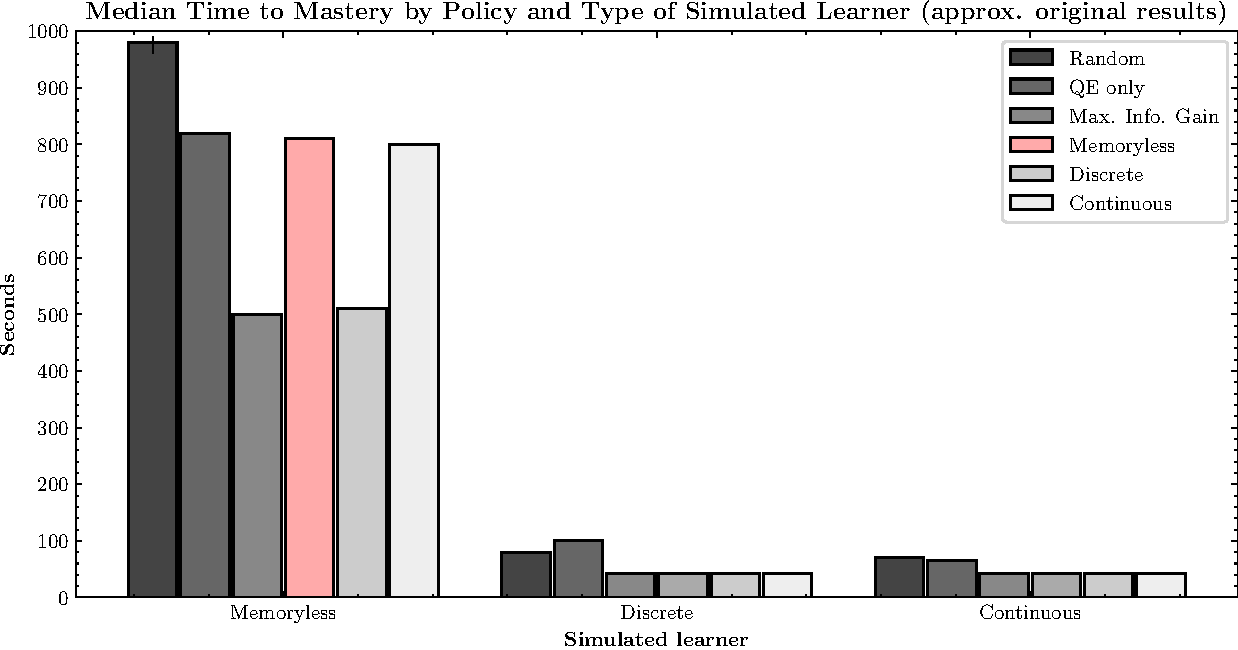
\includegraphics[width=.75\linewidth]{median-time-letter-orig.pdf}
%     \caption{Replicated figure 4 of the original paper for comparison with our results
%     The main difference is highlighted in red.
%     }
%     \label{fig:difference-t1}
% \end{figure}

\begin{figure}[h]
    \centering
    \begin{subfigure}{1\linewidth}
        \centering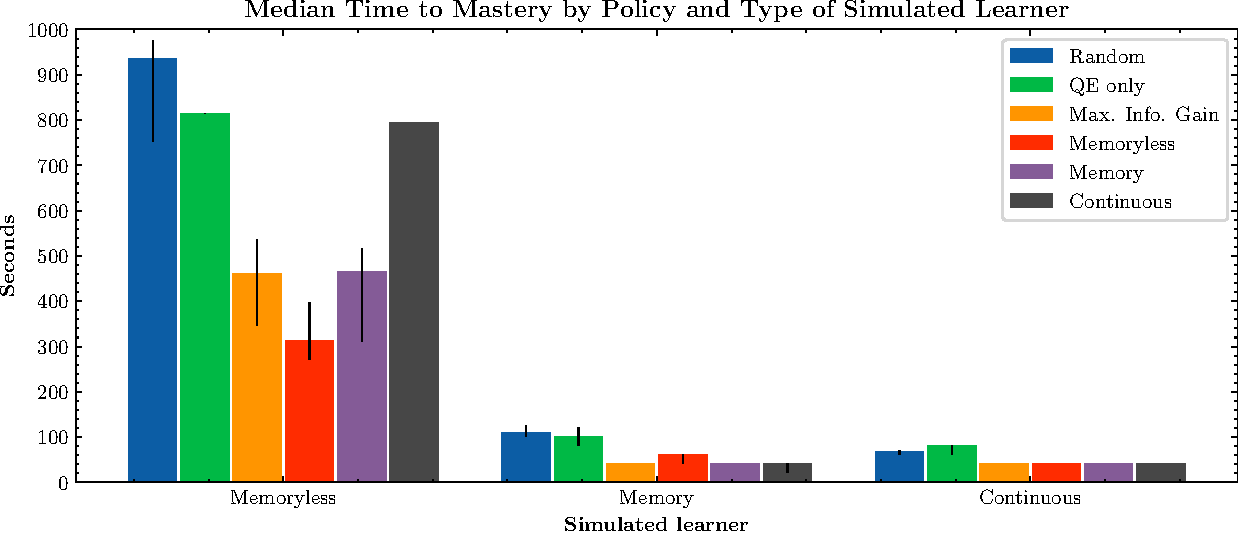
\includegraphics[width=1\linewidth]{figures/median-time-letter-pre.pdf}
        \caption{Our results}
    \end{subfigure}%
    \vspace{10pt}
     
    \begin{subfigure}{1\linewidth}
        \centering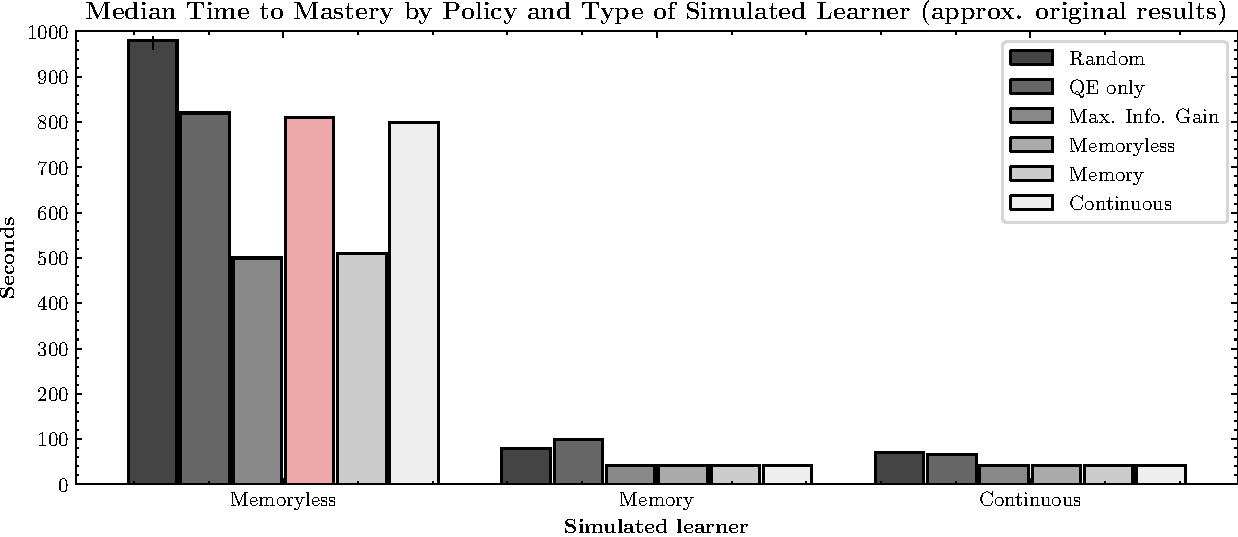
\includegraphics[width=1\linewidth]{figures/median-time-letter-orig-small.pdf}
        \caption{Original results, recreated from the original figure 4. The main difference is highlighted in red.}
    \end{subfigure}
    
    \caption{Median time to mastery for the letter arithmetic task. The results are grouped for each simulated learner (x axis) showing the performance of the different policies. The error bars represent the bootstrapped 68\% confidence interval.
    }
    \label{fig:median-time-comp}
\end{figure}

Our simulation results are shown in \autoref{fig:median-time-comp} (a).
The overall results of the median time to mastery are very similar to the original paper with some notable differences.
%Exact numbers for the original data are not available, so the values given below are approximated from Figure 4 of the original paper. 

Most notably, the result for the memoryless learner with the memoryless policy differs. It is lowest for the memoryless learner with 323.5s while the original authors reported a time around 810s.

The results for the other learners match the original data closely, the random policies differ slightly.
The results for the three planner and the maximum information gain policies paired with the discrete and continuous learners all have a median of 42.0s (two rounds of example activities). 
Only the memoryless policy for the discrete learner deviates from this value, although it is still contained in its confidence interval.

When comparing the time to mastery for the two random policies, note that the QE only policy might achieve a lower number because the most expensive action is not used.
This can have a negative effect on the learning because with the random policy, there is a $2/3$ chance of seeing evidence, while with QE only, there is only a $1/2$ chance. 
This might explain the higher failure rate for the memoryless learner with the QE only policy.


\begin{table}[h]
    \centering
    \small
    \begin{tabular}{l|rrr|r}
        \hline
        \textbf{Policy} & \multicolumn{2}{l}{\textbf{Failure rate with learner}} & & \textbf{Computation time}\\
                        & Memoryless &  Memory & Continuous &  \\
        \hline
        Random          & 50\% & 0\% & 0\% & - \\
        Random QE only  & 68\% & 0\% & 0\% & - \\
        Max. Information Gain & 32\% & 0\% & 0\% & 0.1s \\
        \hline
        Memoryless      & 22\% & 0\% & 0\% & 1.3s \\
        Discrete memory & 18\% & 0\% & 0\% & 2.2s\\
        Continuous      & 96\% & 26\% & 0\% & 1.2s \\
        \hline
    \end{tabular}
    \caption{Failure rates and mean computation times over 50 simulations for each policy-learner pair.
    %Failure is encountered when the concept is not learned after 40 teaching phases.
    }
    \label{tab:failures-t1}
\end{table}

The failure rate of the different simulations, i.e., how many times a learning session was terminated after 40 rounds of teaching phases before the learner achieved mastery of the concept, are reported in \autoref{tab:failures-t1}. 
It shows that the memoryless learner consistently failed to learn the concept, ranging from 18\%-96\% of the cases.
It is highest with the continuous policy at 96\% and second highest for the QE only policy at 68\%. The median time to mastery is very similar in both cases though since the continuous policy samples only the cheapest activity type (quiz) after some point.
The discrete memory learner only fails with the continuous policy in 26\% of the cases, while the continuous learner never fails to learn.
Although the information is not available in the original paper, we assume that the failure rates are similar since the median time to mastery is very close.



\autoref{tab:failures-t1} shows computation times for the different models across all learners. 
%Pre-planning is well below one minute in all cases. 
%However, only one or two paths are considered, as mostly example actions were planned which have no responses to adapt to. 
The online planning computation times are well below 3 seconds which was put forward as the threshold in the original paper. 
%This means, we could increase the sample sizes and stay within the limit.
Increasing the sample sizes did not produce significantly different results. 
%We tested increasing the sample size to 10 for all models and the results were the same for most of the simulations. The memoryless learner shows slightly different results for the memoryless and discrete memory policy, however, it lied still within the confidence interval of the results above.
%Computing power has increased since the publishing of the original paper, so it seems natural that more samples can be incorporated now.

% \begin{table}[h]
% \centering
% \small
% \begin{tabular}{lr|r}
% \hline
% \textbf{Model}  & \textbf{Planning Samples}    & \textbf{Mean computation time}  \\
% \hline
% Max. Info. Gain & 15     & 0.1s                  \\
% \hline
% Memoryless      & 7, 6            & 1.3s                  \\
% Discrete memory & 8, 8            & 2.2s                  \\
% Continuous      & 4, 3            & 1.2s                  \\
% \hline
% \end{tabular}
% \caption{Planning times for different models for the letter arithmetic task.
% %All learner models employ a planning horizon of 2.
% %The two numbers in the samples refers to the number of samples at the first and second tree level. 
% %The max. information gain model only plans one step ahead.
% %and tests all items with the example type.
% }
% \label{tab:times-t1}
% \end{table}

\begin{figure}[h!]
    \centering
    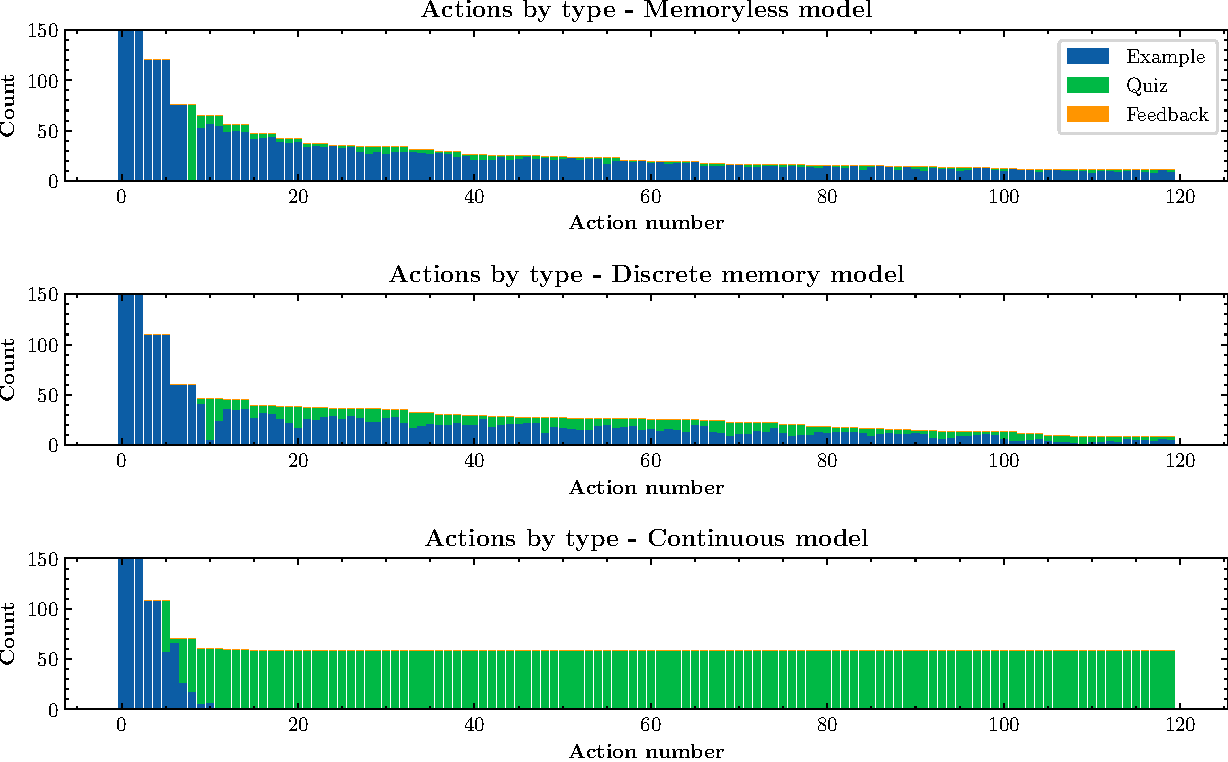
\includegraphics[width=\linewidth]{figures/letter-actions-pre.pdf}
    \caption{Planned activity types per step for each planning model for the letter arithmetic task. 
    %Example actions were predominantly chosen in the discrete models, while the continuous model planned mainly quiz actions after a few steps.
    }
    \label{fig:actions-t1}
\end{figure}

\autoref{fig:actions-t1} shows the teaching activity types planned for each model.
Both the memoryless model and the discrete memory model planned mainly example activities.
Interestingly, both sampled a quiz type after eight and nine example types.
Afterwards, the discrete memory model employed more quizzes than the memoryless model.
The continuous model started with example activities only but gradually used more quiz type actions which were the only type used after action step 12.
No model planned feedback activities.


We provide data tables of the results in the supplementary section \ref{sec:supp}.

\subsubsection{Number game}

% \begin{figure}[t]
%     \centering
%     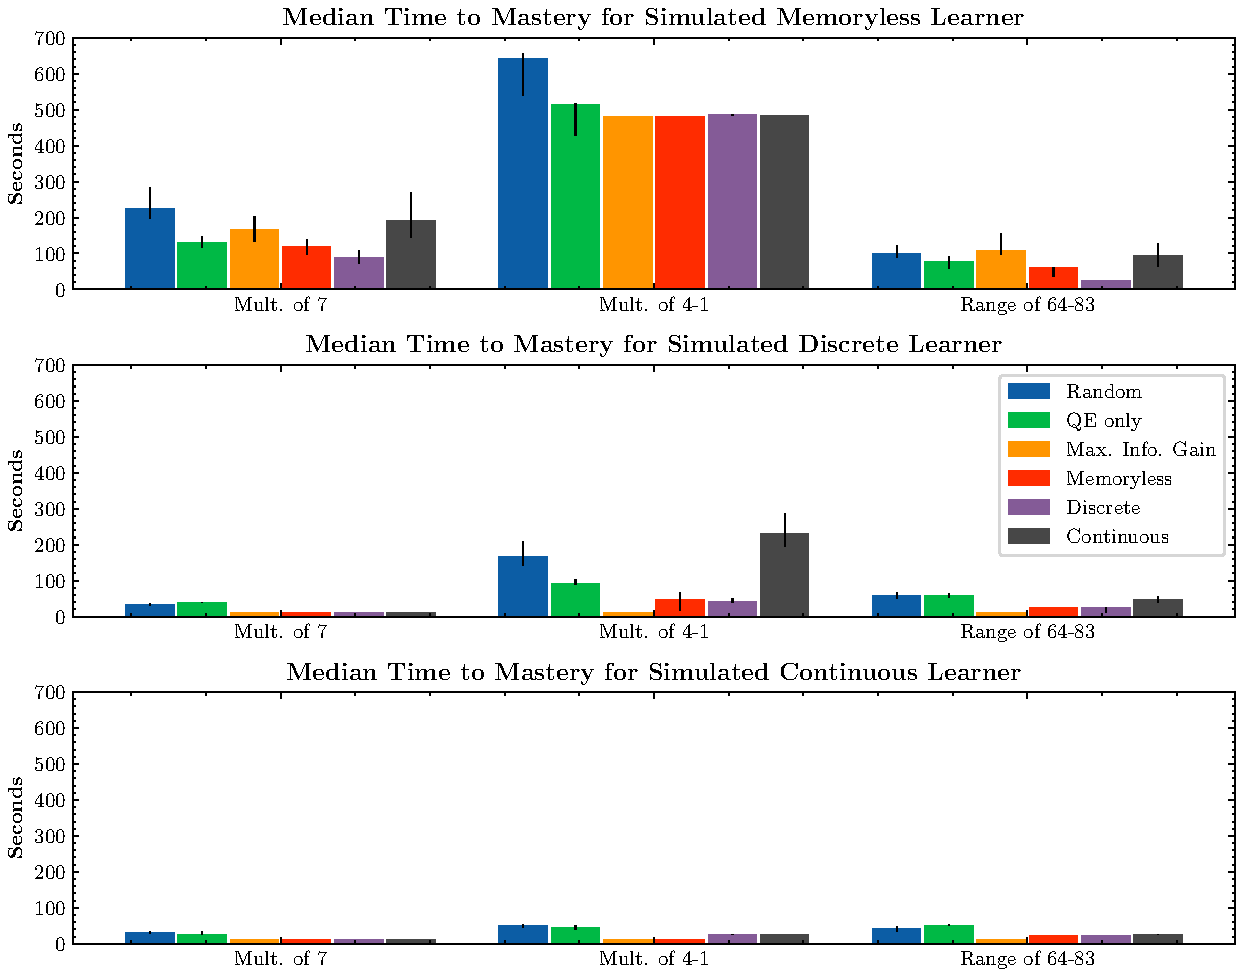
\includegraphics[width=\linewidth]{median-time-ng-combined.pdf}
%     \caption{Median time to mastery for the number game separated for each simulated learner and grouped by task. 
%     Error bars represent bootstrapped 68\% confidence intervals. 
%     Comparable to figure 9 of the original paper.}
%     \label{fig:median-time-ng}
% \end{figure}


% \begin{figure}
%     \centering
%     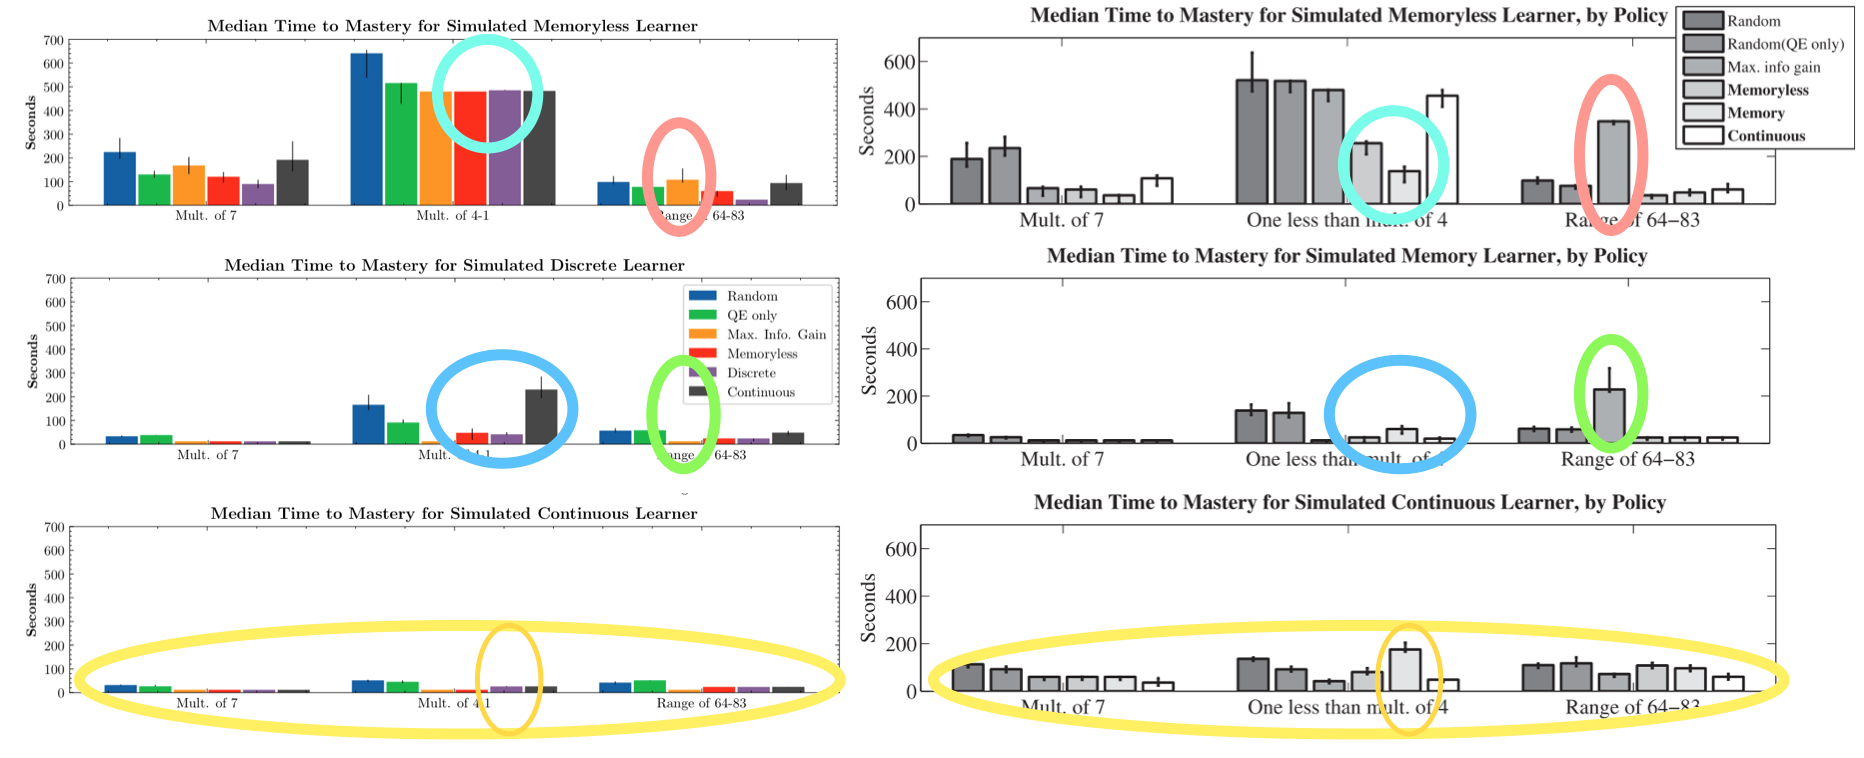
\includegraphics[width=\linewidth]{replication-diff-number-game.png}
%     \caption{Replication difference for the number game between our results (left) and the original data (right).
%     }
%     \label{fig:difference-t2}
% \end{figure}


\begin{figure}
    \centering
    \begin{subfigure}{.9\linewidth}
        \centering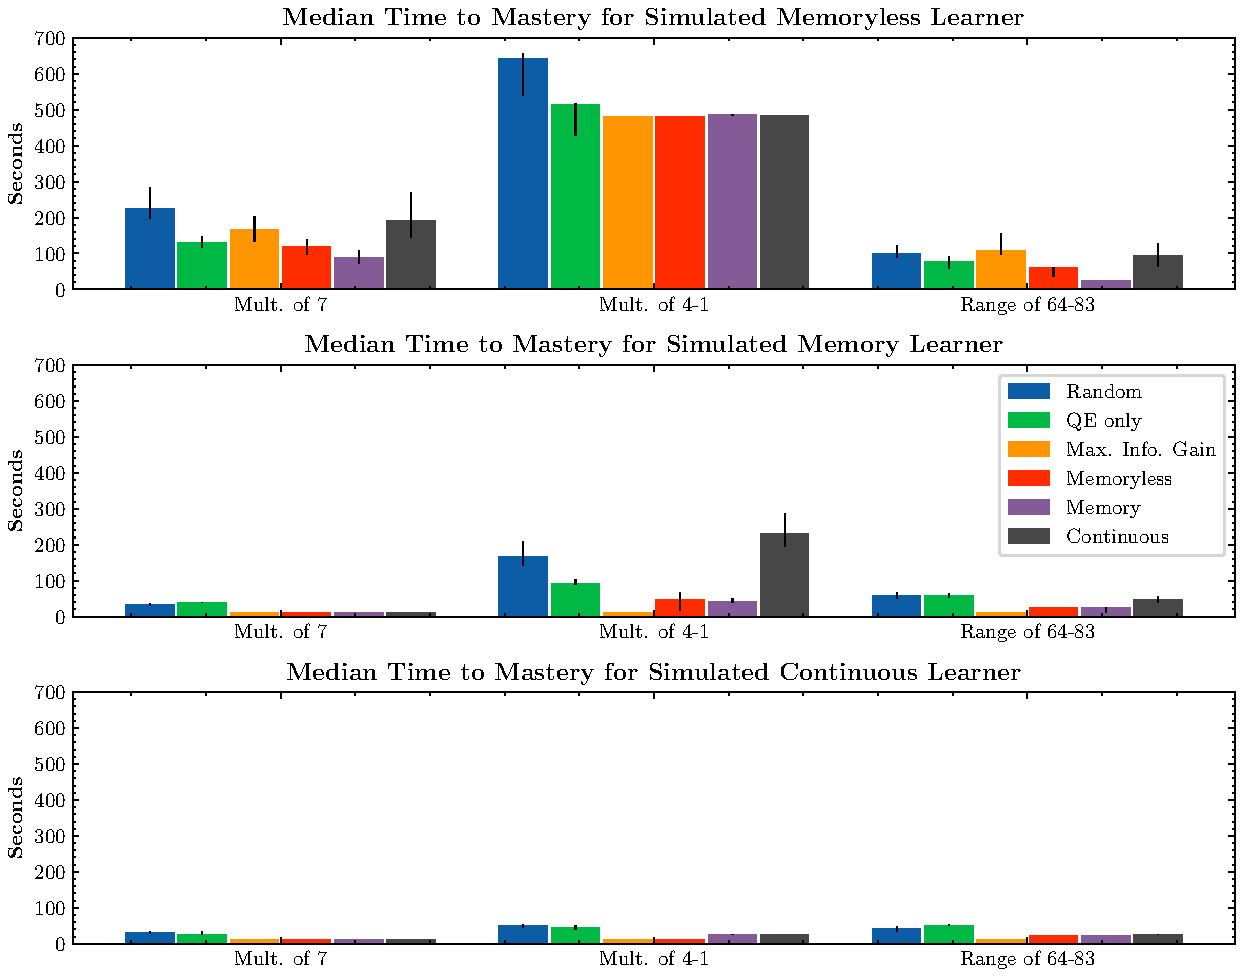
\includegraphics[width=1\linewidth]{figures/median-time-ng-pre.pdf}
        \subcaption{Our results}
    \end{subfigure}
    \vspace{10pt}
     
    \begin{subfigure}{.9\linewidth}
        \centering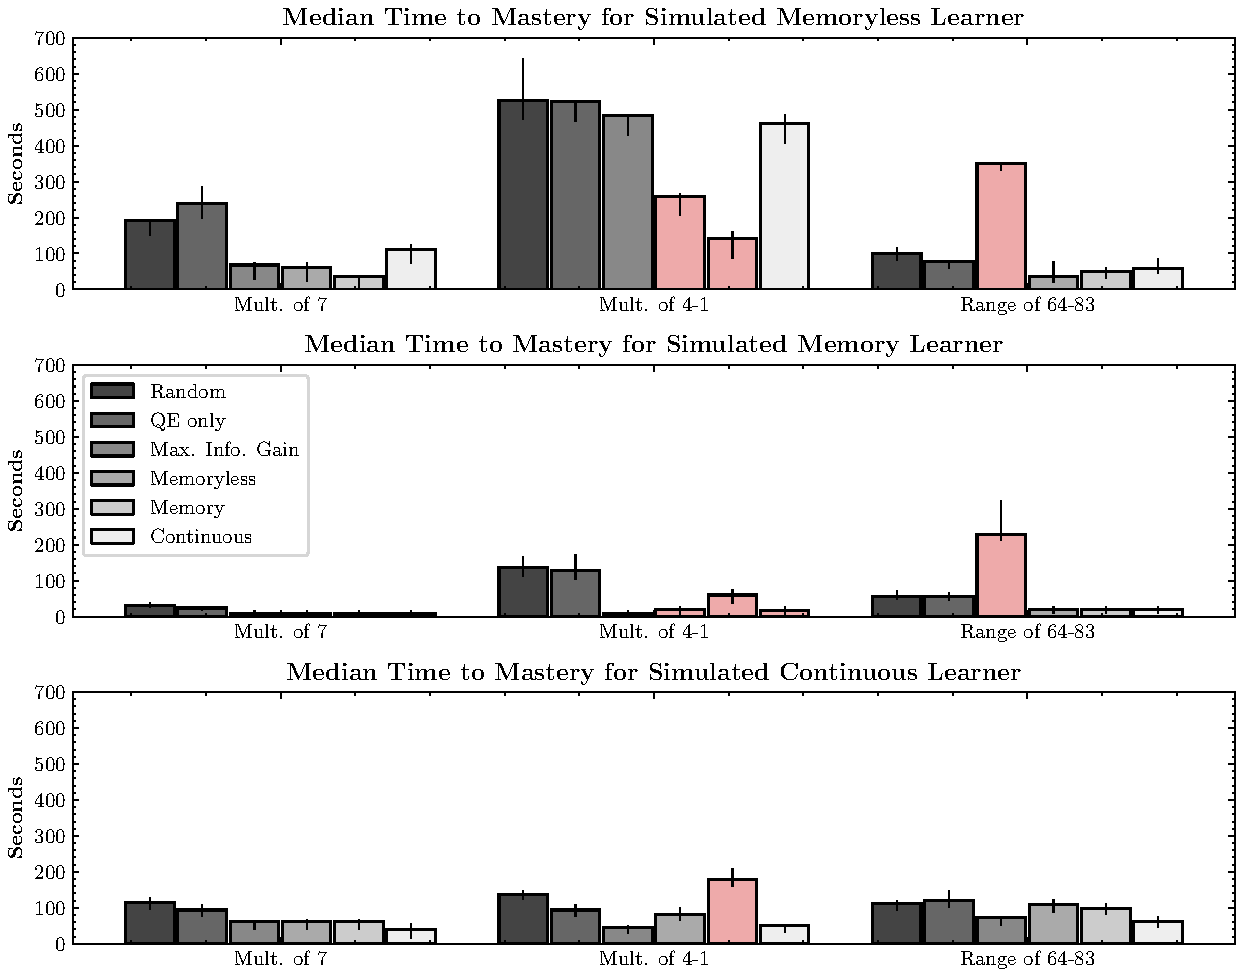
\includegraphics[width=1\linewidth]{figures/median-time-ng-orig.pdf}
        \subcaption{Original results, recreated from original figure 9. Major differences are highlighted in red \\ ($\Delta \geq 50\%$ and relative performance to other policies differs).
        }
    \end{subfigure}
    
    \caption{Median time to mastery for the number game separated for each simulated learner and grouped by task. 
    Error bars represent bootstrapped 68\% confidence intervals. 
    % \textit{Top}: Our results. \textit{Bottom}: Original results, recreated from figure 9 from original paper.
    % TODO define major difference
    }
    \label{fig:median-time-ng-comp}
\end{figure}


Our results are shown in \autoref{fig:median-time-ng-comp} (a). 
The overall structure of the results appear similar to the original results but there are major differences in our data.
We consider differences major if the values differ at least 50\% and the relative performance compared to the other policies is different.

For the simulated memoryless learner (top chart), our results for the target \textit{multiples of 7} are slightly higher and not clearly better than the random policies while their relative performance matches the previously reported results.
For the target \textit{multiples of 4 minus 1}, our results with the memoryless planner and the discrete memory planner differ significantly. 
Our simulations resulted in a median time to mastery of ~480s for both which was reported as ~260s and ~140s in the previous work. 
Hence in our results, no planner exhibits a high performance while previously, the discrete planners resulted in low teaching times.
In the target \textit{Range of 64-83}, we find the maximum information gain policy performs comparable to the continuous policy at 108s while it performed significantly worse than the other planners at ~350s in the original results.

For the simulated discrete memory learner (middle row), with the target \textit{multiples of 4 minus 1}, our continuous planner resulted in a significantly worse performance than all other policies which performed remarkable in the previous paper.
For target \textit{Range of 64-83}, our maximum information gain policy achieves a very high performance with 12s, while in the original results, it was significantly worse than all the other policies with ~230s.

For the simulated continuous learner, we find it to perform significantly better with all targets and with all policies, achieving the best results among the different learners, and not allowing to distinguish between the planners' performance. 
In the original work, the continuous learner was outperformed in many cases by the discrete memory learner and even sometimes the memoryless learner.
For the target \textit{multiples of 4 minus 1}, our policy based on the discrete memory policy performed equally well to the continuous policy with ~26s, while it was previously reported with a performance of ~180s, much higher than the other policies.

In general, we note that our results do not follow a clear line in comparison to the original data.
The best policy for a learner-policy pair is often different in our simulations even if the differences are not large.


\begin{table}
    \centering
    \small
    \begin{tabular}{l|rrr|rrr|rrr|r}
        \hline
        \textbf{Policy} & \multicolumn{3}{l|}{\textbf{Multiples of 7}}  & \multicolumn{3}{l|}{\textbf{Mult. of 4 minus 1}} &  \multicolumn{3}{l|}{\textbf{Range 64-83}} & \textbf{Comp.} \\
                        & Mless & Mem & Cont & Mless & Mem & Cont & Mless & Mem & Cont & \textbf{time} \\
        \hline
        Random          & 12\% & 0\% & 0\% &            54\% & 2\% & 0\% &      2\% & 0\% & 0\% & - \\
        QE only         & 6\% & 0\% & 0\% &            54\% & 2\% & 0\% &      0\% & 0\% & 0\%  & - \\
        \makecell[l]{Max. Info. \\ Gain} & 16\% & 0\% & 0\% &             72\% & 6\% & 0\% &      6\% & 0\% & 0\%  & 0.2s \\
        \hline
        Memoryless      & 4\% & 0\% & 0\% &            70\% & 0\% & 0\% &      0\% & 0\% & 0\%  & 3.7s \\
        Memory          & 4\% & 0\% & 0\% &            70\% & 0\% & 0\% &      0\% & 0\% & 0\%  & 2.4s \\
        Continuous      & 28\% & 0\% & 0\% &           68\% & 18\% & 0\% &       0\% & 0\% & 0\%  & 21.9s \\
        \hline
    \end{tabular}
    \caption{Failure rates and computation times over 50 simulations for the number game tasks. }
    \label{tab:failures-t2}
\end{table}

\autoref{tab:failures-t2} shows the failure rates for the second experiment. 
We note similar results as in the first experiment: The memoryless learner fails to learn in some cases, especially for the target \textit{multiples of 4 minus 1}. In fact, the failure rates are very similar across all planners.
In that task, also the discrete memory learner fails to learn with the random, maximum information gain and continuous policies.
However, the failure rates are lower than in the first experiment.
The continuous learner never fails to learn.


% \begin{table}
% \centering
% \small
% \begin{tabular}{l|r}
% \hline
% \textbf{Model}  & \textbf{Mean computation time}  \\
% \hline
% Max. Info. Gain & 0.2s                  \\
% \hline
% Memoryless      & 3.7s                  \\
% Discrete        & 2.4s                  \\
% Continuous      & 21.92s                  \\
% \hline
% \end{tabular}
% \caption{Planning times for different models for the number game.}
% \label{tab:times-t2}
% \end{table}

The computation times are reported in table \ref{tab:failures-t2} in the last column. 
They are significantly higher than in the first experiment and close or larger than the threshold of 3s. 
In particular, the continuous policy exhibited a mean computation time of more than 20s since it was planning three horizons into the future.
%%% Lukas: In the first task the runtime was never an issue, so I didnt do the cutoff after 3s like they described in the paper. Now I'm thinking for this task it could produce some differences - however overall, for the continuous model the results are close in most cases and rather worse despite the possibly larger search. What do you reckon?
The higher computation times make sense considering that the state space is around 7 times larger than in the letter arithmetic task\footnote{The precomputation times were sometimes significantly higher for the number game, depending on the number of quizzes it sampled in the first 20 steps. This resulted in some cases in over 5,000 paths to be precomputed and a runtime of more than 10 hours. In most cases though, the number of evaluated paths was below 10 and done in few minutes.}.
Note though that we invested less effort into making the computations efficient for the number game.

\begin{figure}
    \centering
    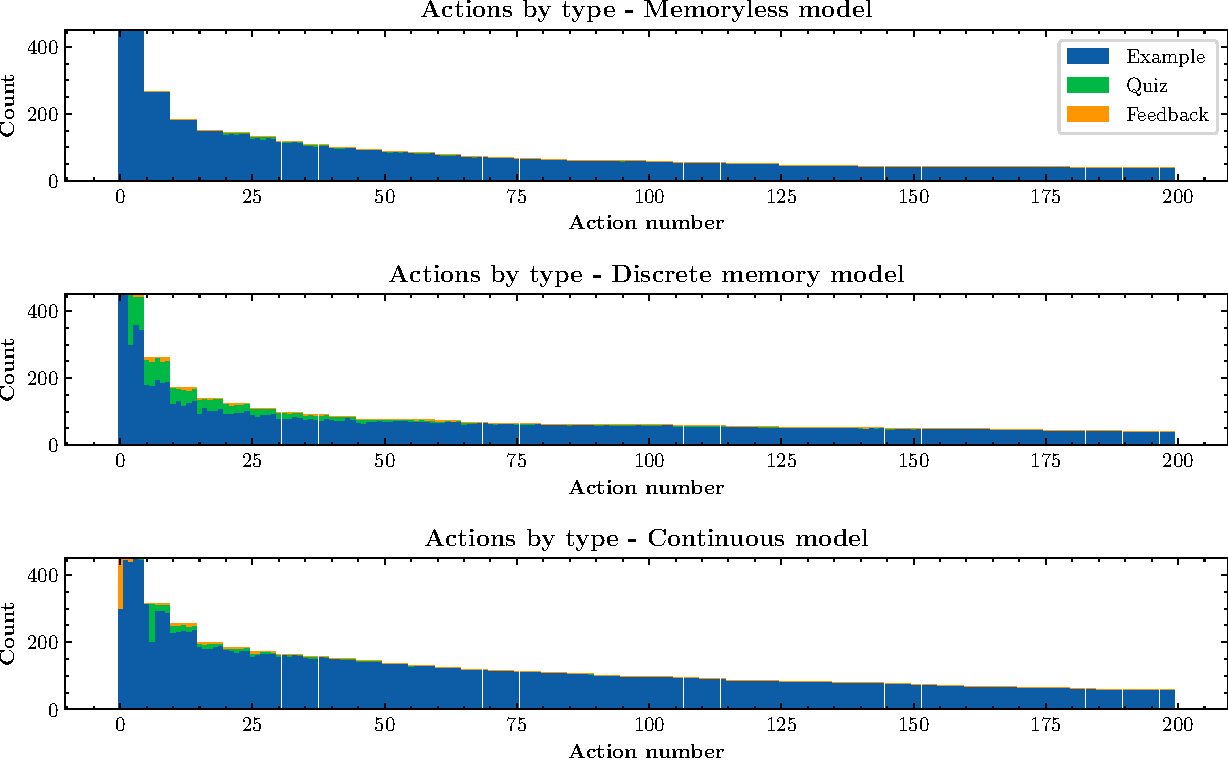
\includegraphics[width=\linewidth]{figures/ng-actions-pre.pdf}
    \caption{Planned teaching activity types per step for each planning model for the number game. 
    %Example actions were predominantly chosen.
    }
    \label{fig:actions-t2}
\end{figure}

Finally, \autoref{fig:actions-t2} shows the sampled teaching types for the different models, combined for all three tasks.
Recall that in the number game, the cheapest action type was the example action.
We notice that it is strongly dominated by example actions in all planners.
The discrete memory and the continuous model sometimes planned feedback actions and quiz actions.

Again, detailed results and statistics are provided in the supplementary section \ref{sec:supp}.

\subsection{Implementation}

We implemented the model in Python 3, using Numpy to perform many calculations in vectorized form.
Simulations are run in parallel to reduce the needed execution time. 
Reproducibility is achieved by using fixed seeds for the random number generators in Python and Numpy. 
The code is publicly available on GitHub at \url{https://github.com/luksurious/faster-teaching/}. 
All possible execution modes are configurable via command-line arguments which also allows a manual learning mode for diagnosis. 

All simulations were executed on Ubuntu 18.04 with Python 3.7.5 on an Intel(R) Xeon(R) CPU E5-1650 v4 @ 3.60GHz and 32GB of RAM.

To improve performance, the belief update is always performed separately for refinement and evidence activities as described before. 
Further, the planning algorithm is slightly improved to stop the iteration over possible observations if the current cost of the action is already higher than the currently known best value.
% Note though, that the code for the letter arithmetic task is more optimized than the code for the number game.

To handle edge cases where a belief contains zero probability for all concepts (usually due to inconsistent responses), we reset the belief in the discrete models to the initial belief, similar to the particle depletion case in the particle filter implementation.

%In the random policy, to achieve a sensible baseline, we ensure that the same item is not used in a single teaching phase.

The biggest difference to the original implementation is that we did not employ the limit on the computation times to 3s since we did not perform a user study.


\section{Discussion}

\subsection{Results}
We were able to partially replicate the results reported by Rafferty \textit{et al.} for the simulated learners.
Indeed, the overall picture is similar but some results are different that lead to a different evaluation.

We encountered two main differences in our replication. First, in the letter arithmetic task, the memoryless policy performed significantly better with the simulated memoryless learner. Intuitively this makes sense because it is matching the cognitive model between the planner and learner.
Second, in the number game, the maximum information gain policy achieved comparable performance to the POMDP policies where it was previously reported to be greatly outperformed by them.


Certainly, the random policies were not good teachers.
However, the policy based on the maximum information gain achieved comparable results to the other POMDP policies, while mostly failing in the original paper. 
% We did not find it to be failing as in the original paper.
% Since it also employs the continuous belief model inside to trace the state of the learner, we argue that it should still be considered as a POMDP policy rather than a baseline.
%Considering the computational costs of the forward search planning, it appears to be a reasonable and low-cost approach.
% Even so, the computation times with the other policies is not comparable because it only searches over a horizon of one instead of two or three.
Since it also employs the continuous belief model inside to trace the state of the learner, it would be interesting to see whether reducing the horizon of the other models leads to similar performance (with better runtimes) and if the maximum information gain policy can be further improved by increasing the horizon.

%In many cases, the difference between the POMDP models are not large, so considering the computational requirements, it seems that the more conservative and simple memoryless model would be a good choice for practical applications. 
%Overall, the memoryless model achieves the best scores considering the different types of learners together.


Our results show that for a strong learner, the planning model is not very important as all achieve high performance. 
For a weaker learner, our simulations show that a policy with weaker learning assumptions fits best.
%While it was possible to show that the model is able to plan better than a random model, it seems too simple to really evaluate the the models as the baseline using only example actions based on the maximum information gain achieves the same results in terms of median time to mastery as the more sophisticated POMDP models.
The letter arithmetic does not allow to draw conclusions as all planning policies perform equally well.
In the number game, the results are more differentiated but it is still not possible to draw clear conclusions about the suitability of a policy and whether they are superior to the maximum information gain policy.

Even though the continuous policy was the only one to use a horizon of 3 in the number game which resulted in much higher computation times, its results for mismatching simulated learners were worse than in the original paper. This might be due to our implementation not stopping calculations after 3 seconds. If that is one reason it might imply that an improved search might actually be counter-productive in these cases.

% In the number game, we find it surprising that the horizon for the continuous model was set to three with similar sample sizes as the discrete models that only search two levels. 
% This is in contrast to the settings of the first task where all models used the same horizon and the continuous policy sampled fewer items.
% Considering that the state space is around 7 times larger in the number game than in the letter arithmetic tasks, it is counter-intuitive to largely increase the search space.
% As a result, we show that the computation times in this case is significantly increased, well above a reasonable threshold of three seconds.

% model discussion
\subsection{Learner models}

Our results provide extra information regarding the failure rates to evaluate the policies.
The mastery time alone can be misleading as it might mask failure rates with cheap actions as it is the case with the continuous policy in the first task. 
From this analysis we found that the simulated memoryless learner often fails to learn the concept and as such it seems not a very plausible model for human concept learning. We deduce from the original paper that the human learners were able to mostly learn the concepts correctly in contrary.
On the other side, the continuous policy most often led to failures in the learners, indicating that it is not well suited for different types of learners.
This can also be seen from the types of actions sampled. In the letter arithmetic task, it converged to choose only quiz activities. This fails to give new evidence and correct mistakes, and resulted in the high failure rate for the memoryless learner.
This is in line with the analysis by Rafferty \textit{et al.} that the continuous policy overestimates the learning capabilities and might not discover a divergence between the belief and the true state.

The two discrete models (memoryless model and model with memory) could be improved by assigning higher transition probabilities to states that are closer to the current state.
%Especially in the memoryless model, the transitions to new states is a random guess based only on the current information. 
% In an MDP, states can contain information about the history and transitions often depend on the current state, e.g., favoring transitions to states that are closer to the current state. 
% The same can be applied here: as the current state contains information about the previous action, we can exploit this information without keeping an explicit history by assigning higher probability to states with less distance to the current state. 
For example, in the letter arithmetic task, the distance can be measured by the number of necessary pairwise changes to move from one state to another. 
We argue that this also better reflects human learning. 
%Integrating this into the learner model can improve the performance significantly for cases with related states.
%(see \autoref{sec:supp}) and renders the memoryless model actually usable. 
% In larger domains, it would also make convergence to the target state more likely as the implicit history inside the state is better utilized.

Further, the discrete model with memory assumes a perfect memory. 
It seems plausible that this is not always the case for human learners and might be too strong of an assumption. 
However, if different memory state possibilities were integrated into the model, the state space would increase significantly, reducing its tractability. 
Nevertheless, it could be a reason for the high transition noise determined for this learner model in the letter arithmetic task.


% task discussion

% \subsection{Tasks}




%Yet, already for this simple problem, the planning horizon was very short because the computational requirements increase exponentially and increasing the horizon makes it unusable in a live setting.


\subsection{Framework}
%%% Lukas: I might be discussing too much?
One key to implementing the models efficiently is to not use the explicit Bayesian belief update equation but instead treat the belief update separately for inferring the learner's previous state and for calculating transitions based on new evidence, mainly in the case of feedback activities.
The formulation as a POMDP could be improved by taking this into account or employing different action types that fit the structure better.


% framework discussion

% teaching goal, cost definitions
Defining the teaching goal and associated rewards or costs is a critical part in this framework.
Focusing on shortest time and associating the average time to process an action type nearly eliminated one of the teaching types (feedback type), presumably due to the high costs associated. 
It was shown that the continuous model converges to the cheapest action type and the differences in costs between the first and second task resulted in a very different behavior of the model.
As the main planning decision, as stated in the original paper, can be seen as deciding between teaching new content (examples) versus inferring the learner's state (quizzes), defining the cost function in the current way does not seem to facilitate this decision well enough. 


% leaf estimation
The estimation of leaf nodes requires more evaluation. 
The dimension $\alpha$ in the formula needs to be scaled appropriately to the state space and corresponding changes in success probability from teaching actions. 
Otherwise, the forward search could lead to mainly choosing the cheapest action if the success probability of the correct concept is too small in comparison.
%%% Lukas: Should I add an example? It is a rather simple calculation but a bit tricky to explain in short words.
%\footnote{A simple calculation. Assume the cheapest action type quiz has a cost associated of 4, this means the success probability in the leaf calculation is scaled by 40. When choosing a quiz, the learner's state does not change. .... p(true)= 1e-6. With quiz 1 horizon, val = 4+40*1e-6=4.00004. Example costs 5 and pushes to true concept, p(true)=1e-5. Val = 5+40*1e-5=5.0004. With uniform observation probability. this actually happens in the number game for the most unlikely concept (multiples of 4 minus 1) if the values of the first task are taken}
It would be interesting to see if the estimation of leaf nodes correspond to the true values of the states in the experiments.

% future
%These costs are highly important but remain fixed for all participants even though it seems plausible that different learners exhibit different learning times. 
%In a real experiment, it would be interesting to see if adapting the costs of the actions to the historical data taken by that user would adapt better to the individual and possibly make feedback types more attractive to use. 

%Possibly adapt the estimation function accordingly to fit the data.
%Similar data and user-based adaptation could be performed for the noise parameters to adapt to the individual learners.

% assessment phase, determining goal state
% how is it done in "regular POMDPs"? shouldnt either the belief determine if the agent stops (i.e. cont. model stops even if not learned), or it is a separate action/observation which would then be integrated into the model and belief updates??
Having a separate assessment phase whose purpose is solely to determine if the teaching is finished, and not using the responses to tune the belief, falls outside of the POMDP formulation and appears counter-intuitive. 
This results in a few cases where the teacher is not able to determine the wrong hypothesis of the learner when the belief diverges from the state, and no quiz actions are planned to validate the belief. 
It would be interesting to see if integrating the assessment as a separate action type into the planning algorithm would solve this issue.
% In a human experiment, the assessment phase might also give additional information about the concept to be learned (e.g., in the number game) as learners might assume that some should be from within the concept.
%Integrating the assessment phase into the planning model could alleviate these issues and enforce more regular "sanity checks" as otherwise the teaching would not terminate.



% formulation as POMDP still interesting, although concrete tasks and learner models seem in need of adjustment



\section{Conclusion}
Formulating teaching as a POMDP is a useful approach that allows to use sophisticated planning algorithms with cognitive learner models.
% We replicated the work by Rafferty et al. with some differences.
% , and also clarified the formulation in a more rigorous way.
% In the proposed context of concept learning, there is no clear differentiation in terms of performance between the different learner models and the policy based on the continuous model with maximum information gain.
% For further application, we argue that the optimization goal and cost definition should be formulated differently to produce be more robust and address the issue of learning failure.
% Further, 
While computational challenges remain for employing the proposed method in real-time settings, investigating challenges and trade-offs for real-world teaching problems (e.g., second language learning) are still necessary to fully understand the applicability of the formulation.
Through this replication, we hope to facilitate research in this direction as currently employed heuristics in tutoring systems lack adaptability for which model-based systems are promising candidates. % by providing an extended description and a free implementation of the Faster Teaching's algorithm.

\section{Acknowledgements}
We would like to thank Anna Rafferty (the first author of the original paper) for answering our numerous questions and sharing her implementation with us.

\section{Author contributions}
AN and LB designed the replication.
LB implemented the model, performed the subsequent analysis, and wrote the paper. AN supervised the process.
